  \documentclass[a4j,twocolumn]{jsarticle}
  \usepackage[dvipdfmx]{graphicx}
  \usepackage{url}

  \setlength{\textheight}{275mm}
  \headheight 5mm
  \topmargin -30mm
  \textwidth 185mm
  \oddsidemargin -15mm
  \evensidemargin -15mm
  \pagestyle{empty}


  \begin{document}

  \title{旅行計画アプリの開発}
  \author{情報科学科 \hspace{5mm} 37022463 \hspace{5mm} 山本果音}
  \date{}

  \maketitle


\section{序論}
\label{sec:org576a304}
旅行計画の共有ツールとして,Googleマイマップ[1]を利用するケースが増えている.
Googleマイマップは「自分の地図を作成し共有することができる」[1]というニーズに応えるために開発された背景がある.
しかし,Googleマイマップを旅行のプランニング用途で使用する場合,以下のような課題が存在する.
\begin{enumerate}
\item 観光場所を日程ごとに分けて管理する機能が標準では備わっておらず,旅行日ごとの予定が視覚的に把握しづらい.
\item 登録したスポットの訪問順序が地図上で明確に表示されないため,移動の流れが分かりにくい.
\end{enumerate}
結果として,訪問予定の観光地の情報が複数の地図やファイルに分かれてしまい, 全体の予定を整理しづらくなるだけでなく,
家族や友人など旅行メンバーとの共有時に混乱が生じることがあった。
そこで,旅行先の情報を日程や訪問順に沿って視覚的に整理し,家族や友人との円滑な情報共有を促進する旅行プランニングアプリの開発を目指す.



\begin{figure}[htbp]
\centering

\includegraphics[width=7cm]{./figs/discord.jpg}
\caption{\label{fig:org69a908b}Googleマイマップでスケジュールを組んだ時の画面.}
\end{figure}


\section{開発手法}
\label{sec:org7f0e23c}
開発環境としてDjango[2]を選定した.
Djangoの利点は以下の2つである.[3]
\begin{enumerate}
\item 迅速な開発が可能.
\item フォーム作成が容易にできる.
\end{enumerate}
また開発はpythonを用いて開発を行った.





\section{結果}
\label{sec:orgf4fd8a9}
今回開発したWebアプリには,以下のような利点がある.
\begin{enumerate}
\item 旅行日数を入力することで,各日程の項目が自動生成されるため,日付ごとの旅行プランニングが容易になる.
\item 訪問順に番号が付与されることで,旅程の流れを地図上で視覚的に把握しやすくなる.
\end{enumerate}
Googleマイマップでは、旅行日ごとに個別のレイヤーを作成・管理する必要があるため, 観光地や移動ルートなどの情報が複数の地図に分かれてしまい,
全体の予定を一目で把握しづらくなる. また,地図が複数に分かれていることで,旅行メンバーとの情報共有にも手間がかかり,
混乱が生じやすいという課題があった.
これに対し,本アプリでは旅行日程を事前に入力することで,各日程の構成が自動的に整理され,
旅行計画の一元管理と視覚的な理解が可能となる.

\begin{figure}[htbp]
\centering
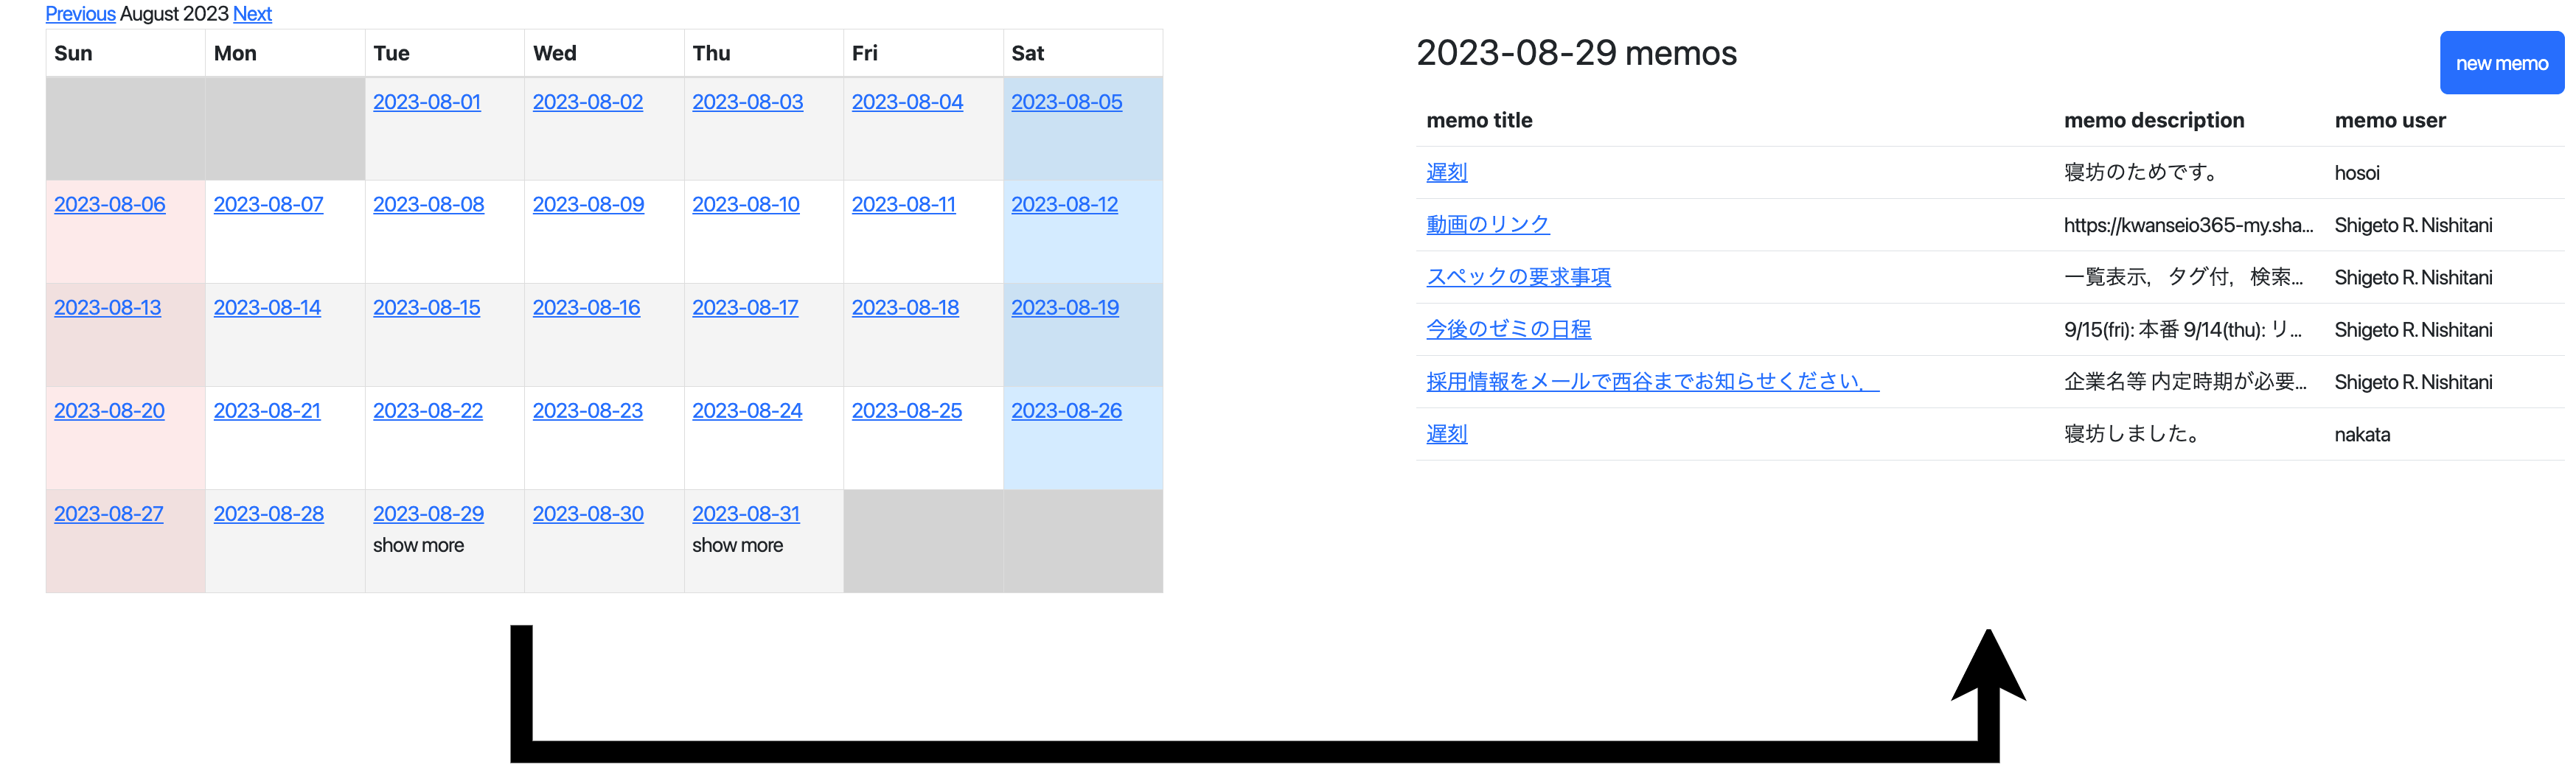
\includegraphics[width=10cm]{./figs/app_motion.png}
\caption{\label{fig:orgf82e9c5}参照したい日付に保存されたデータを参照する一連の動作.}
\end{figure}


\section{今後の課題}
\label{sec:org88af1da}
今回は基本的なCreate(生成),Read(読み取り),Update(更新),Delete(削除)処理(CRUD処理)に加えて,
データの絞り込み機能,グループ作成,メンバー招待・参加機能を開発した.
今後は共有データの見逃しを防ぐための通知機能,ローカルPC上で作成したメモから
このWebアプリへの送信スクリプトを開発する.
また,閲覧回数などの要素から共有データを重みづけし,不要なデータは自動的に削除する機能も組み込み,
更なる共有データの整理,Webアプリのパフォーマンス向上を図る.


\small\setlength\baselineskip{10pt}
\begin{thebibliography}{9}

\bibitem{Google My Maps} Google マイマップ,\url{https://www.google.co.jp/intl/ja/maps/about/mymaps/}.
\bibitem{Django}Djangoドキュメント,\url{https://docs.djangoproject.com/ja/5.1/topics/}.
\bibitem{Django}Djangoの概要 ,https://docs.djangoproject.com/ja/5.1/intro/overview/.
\end{thebibliography}
\end{document}
